\documentclass[conference]{IEEEtran}
\usepackage{blindtext, graphicx}

% Add the compsoc option for Computer Society conferences.
%
% If IEEEtran.cls has not been installed into the LaTeX system files,
% manually specify the path to it like:
% \documentclass[conference]{../sty/IEEEtran}



% correct bad hyphenation here
\hyphenation{op-tical net-works semi-conduc-tor}


\begin{document}
%
% paper title
% can use linebreaks \\ within to get better formatting as desired
\title{Biometric Patterns on Hooded Norway rats}


% author names and affiliations
% use a multiple column layout for up to three different
% affiliations
\author{\IEEEauthorblockN{Michael Shell}
\IEEEauthorblockA{School of Electrical and\\Computer Engineering\\
Georgia Institute of Technology\\
Atlanta, Georgia 30332--0250\\
Email: http://www.michaelshell.org/contact.html}
\and
\IEEEauthorblockN{James Kirk\\ and Montgomery Scott}
\IEEEauthorblockA{Starfleet Academy\\
San Francisco, California 96678-2391\\
Telephone: (800) 555--1212\\
Fax: (888) 555--1212}}




% make the title area
\maketitle


\begin{abstract}
%\boldmath
%\blindtext[1]
bla bla bla
\end{abstract}
% IEEEtran.cls defaults to using nonbold math in the Abstract.
% This preserves the distinction between vectors and scalars. However,
% if the journal you are submitting to favors bold math in the abstract,
% then you can use LaTeX's standard command \boldmath at the very start
% of the abstract to achieve this. Many IEEE journals frown on math
% in the abstract anyway.

% Note that keywords are not normally used for peerreview papers.
\begin{IEEEkeywords}
Hooded Norway rats,  long-term periods tracking, rat dataset, behaviour analysis.
\end{IEEEkeywords}






% For peer review papers, you can put extra information on the cover
% page as needed:
% \ifCLASSOPTIONpeerreview
% \begin{center} \bfseries EDICS Category: 3-BBND \end{center}
% \fi
%
% For peerreview papers, this IEEEtran command inserts a page break and
% creates the second title. It will be ignored for other modes.
\IEEEpeerreviewmaketitle



\section{Introduction}
%\blindtext



Behaviour analisys is very important because of \cite{weissbrod2013automated}.... 

Animal biometrics \cite{kuhl2013animal} ...

The Long-Evans rats (Hooded Norway rats) are commonly used in cognitive studies \cite{lambert2016natural,guarraci2016exposure,turner2014comprehensive}, frequently these experiments last several weeks or months, hence, especially when several individuals are placed in the same cage, keep tracking of each animal for a long period of time is a challenging task. In order to overcome this drawback usually, the animals are marked in the tail as in \cite{lambert2016natural}. However, the number of possible distinguishable markers is limited, therefore, with the increase in the number of individuals that share the same cage increases, this approach becomes impractical. 

%with a marker which sometimes need to be refreshed.


%\cite{noldus2001ethovision}

%Object identification. EthoVision distinguishes between two animals in the same arena on the basis of size. To distinguish two animals that are the same size, the user can partly color one animal to the same grayness as the background, thus reducing its apparent size (see Fig- ure 8). Color tracking can be used to distinguish more than two animals (up to 16 per arena). If the animals being tracked are the same color, markers can be used to paint blobs on the animals, which the system will be able to track. For more details on color tracking, see the “Object Detection” section above.

%Object detection. To ensure optimal object detection in any experimental setup, EthoVision offers three different object detection methods. Gray scaling is the fast- est. This method defines the animal as all connecting pixels that are both brighter than a low gray scale thresh- old and darker than a high threshold, and it defines the background as all other pixels. The thresholds can either be set manually by the user or be calculated automatically by the program. Gray scaling is a fast detection method (allowing the highest sample rate), but it cannot be used if the same gray scale values are present in both the ani- mal’s image and the background. The third detection method, color tracking, uses the color of the animal The second method, subtraction , first (before the start of the trial) makes a reference image, 

% cognitive experiments,

%In \cite{lambert2016natural} in order to keep tracking of the rats, each animal’s tail was marked with a nontoxic marker \cite{guarraci2016exposure}

%\cite{weissbrod2013automated} 
%To circumvent inherent human constraints, there is a critical need for machine-based tracking and behavioural phenotyping technologies that are applicable toward the analysis of socially interacting groups of animals. Several research teams have developed automated vision-based tracking tools that support behavioural phenotyping of a single individual in its home cage



What is the problem?
Why do we care about this problem?
Is it possible to use the back patterns on hooded Norway rats as fingerprint ( to disguinsh them)?
what should be a good approach?
Is it useful for automatic behavior analysis?



\section{Literature review}
\subsection{Object detection and Tracking}
Shape context \cite{belongie2002shape} ...

idTracker \cite{perez2014idtracker}...

CRIM13 \cite{CRIM13}...
%novel object preference (NOP) task was conducted in two consecutive days. 

%Latency to enter the centre (defined by a 20 cm radius around the objects), latency to explore Object 1 (O1) and latency to explore Object 2 (O2) were recorded. 

%The second day, rats were placed in the OF apparatus with one cricket. Latency to approach the cricket, latency to kill the cricket and latency to eat the cricket were recorded.
  
%All behaviours were videotaped with a video camera and later coded for latency to float, number of floats, duration of floats, latency to dive and number of dives.

%The latency to dive, the number of dives and time spent floating were recorded for the rats housed in the four home-cage environments during the FS task. On the second day of testing, after the animals habituated to the task, latency to dive was significantly different in the four groups (F3,28 = 4.24, P = 0.014) (Fig. 6). 

%Ten animals were randomly assigned to each group and each animal’s tail was marked with a nontoxic marker and refreshed when necessary so individual animals could be followed throughout the study. 

%duration of four months

%Subsequently, each of the ten animal’s behavior was continuously monitored for the entire hour using microsequencing behavioral analysis to determine the frequency and durations of interactions with environmental stimuli, social interactions with cage mates and self-maintenance behaviors such as grooming and resting. 

\section{Dataset}

The dataset is contains images of 60 Long-Evans rats, for each rat we 
selected 10 images that depict completly their hood patterns. Each image has dimension 50x120 pixels.

\textit{Camera description}: color CCD MicrVideo camera. 1/3" CCD, 600 TV lines, 0.0001 Lux, 3.6mm lens: 1.18"x1.18" square.

\begin{figure}[h]
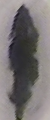
\includegraphics[scale=0.9]{dataset/1.png}
%
\includegraphics{dataset/2.png}

\includegraphics[scale=0.9]{dataset/3.png}
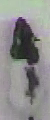
\includegraphics[scale=0.9]{dataset/4.png}

\includegraphics[scale=0.9]{dataset/5.png}
%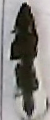
\includegraphics{dataset/6.png}

\includegraphics[scale=0.9]{dataset/7.png}
\end{figure}



Description of the data, what criteria we used and how we selected them.

- show a set of images for the same rat and different views
- show a set of images for different rats (we want to show the variance between rats and changes on the enviroment (eg. variation in illumination)





\section{Conclusion}
%\blindtext




% use section* for acknowledgement
\section*{Acknowledgment}


The authors would like to thank...


% Can use something like this to put references on a page
% by themselves when using endfloat and the captionsoff option.
\ifCLASSOPTIONcaptionsoff
  \newpage
\fi

\bibliography{bibliography}
\bibliographystyle{ieeetr}


% that's all folks
\end{document}


